% ----- Consignes exo 1 ----- %
\begin{td-exo}[Convexité]\,\\ % 1 
	% fill
\end{td-exo}

% ----- Solutions exo 1 ----- %
\iftoggle{showsolutions}{
	\begin{td-sol}[]\,\\ %
		A remplir %TODO solve exercise 1
	\end{td-sol}
}{}


% ----- Consignes exo 2 ----- %
\begin{td-exo}[Convexité]\,\\ % 2 
	% fill
\end{td-exo}

% ----- Solutions exo 2 ----- %
\iftoggle{showsolutions}{
	\begin{td-sol}[]\,\\ %
		A remplir %TODO solve exercise 2
	\end{td-sol}
}{}


% ----- Consignes exo 3 ----- %
\begin{td-exo}[Convexité]\,\\ % 3 
	% fill
\end{td-exo}

% ----- Solutions exo 3 ----- %
\iftoggle{showsolutions}{
	\begin{td-sol}[]\,\\ %
		A remplir %TODO solve exercise 3
	\end{td-sol}
}{}


% ----- Consignes exo 4 ----- %
\begin{td-exo}[Jeu de Slither]\,\\ % 4 
	Le \emph{jeu de Slither} se joue sur un graphe connexe, noté \(G\).
	Chaque joueur choisit à son tour un sommet \(v_i\) non
	précédemment choisi. La suite \(v_0,v_1,\ldots\) doit former un chemin,
	c'est-à-dire que tout pour tout \(i=1, 2,\ldots\),  \(v_i\) doit être
	choisi comme adjacent à \(v_{i-1}\). Le joueur qui ne peut plus 
	jouer a perdu.

	Montrer que si \(G\) admet un couplage parfait alors le second joueur
	a une stratégie gagnante. Montrer que si \(G\) n'admet pas un 
	couplage parfait alors le premier joueur a une stratégie gagnante
\end{td-exo}

% ----- Solutions exo 4 ----- %
\iftoggle{showsolutions}{
	\begin{td-sol}[]\,\\ %
		A remplir %TODO solve exercise 4
	\end{td-sol}
}{}


% ----- Consignes exo 5 ----- %
\begin{td-exo}[Tous d'un coup]\,\\ % 5 
	Soit \(G = (X\cup Y, E)\) un graphe biparti de bipartition \((X, Y)\)
	avec \(\Delta(G) \geq 1\).
	\begin{enumerate}
		\item Montrer que \(G\) admet un couplage couvrant tous les sommets de \(X\) de degré \(\Delta(G)\).
		\item Montrer que \(G\) admet un couplage couvrant tous les sommets de \(G\) de degré \(\Delta(G)\).
		\item En déduire qu'il est possible de partitionner les arêtes de \(G\) en \(\Delta(G)\) couplages.
	\end{enumerate}
\end{td-exo}

% ----- Solutions exo 5 ----- %
\iftoggle{showsolutions}{
	\begin{td-sol}[]\, %
		\begin{enumerate}
			\item On note \(k = \Delta(G)\). Soit \(S\subseteq X_\Delta\).
			On note \(Z = N_G(S)\). On va compter \(e\) le nombre d'aretes
			entre \(S\) et \(Z\):
			\begin{equation*}
				e = \sum_{s\in S} \deg(s) = k\cdot|S|
			\end{equation*}
			Par ailleurs, comme toute arete comptée est incidente à
			un sommet \(z\), on a:
			\begin{equation*}
				e \leq \sum_{z\in Z} \deg(z) = k\cdot|Z| 
			\end{equation*}
			Donc \(k\cdot|S| \leq k\cdot|Z|\) d'où \(|S| \leq |Z| = |N_G(S)|\).
			Par le théorème de Hall, \(G\) admet un couplage qui sature \(X_\Delta\).

			\item Par la question précédente il existe un couplage \(M_X\) saturant
			\(X_\Delta\). De même, il existe un couplage \(M_Y\) saturant
			\(Y_\Delta\). On va extraire de \(M_X\cup M_Y\) un couplage \(M\)
			saturant \(X_\Delta \cup Y_\Delta\). On construit \(M\) en
			regardant chaque composante connexe de \(M_X \cup M_Y\).

			Soit \(C\) une composante connexe de \((V, M_X \cup M_Y\)) (\(C\)
			est soit un chemin soit un cycle).
			\begin{itemize}
				\item Si \(C\) est un cycle
				% insert graph here
				alors on choisit \(M = M_X\) ou \(M = M_Y\) (les deux conviennent)
				et on continue à saturer les sommets de \(C\)

				\item Si \(C\) est un chemin
				% insert graph here
				on peut supposer que sa première arête est dans \(M_X\).
				% inserer 3 graphs disjonction de cas
				On note \(C = x_1 x_2 \ldots x_k\). On a trois cas:
				\begin{enumerate}
					\item Si \(x_1\in Y_\Delta\), c'est impossible car \(x_1\) doit 
					être incident à une arête de \(M_Y\),
					\item Si \(x_1\in Y \setminus Y_\Delta\), on prend \(M = M_Y\),
					\item Si \(x_1\in X_\Delta\) on prend \(M = M_X\).
				\end{enumerate}
			\end{itemize}
		\end{enumerate}
	\end{td-sol}
}{}


% ----- Consignes exo 6 ----- %
\begin{td-exo}[Famille couvrante de cycles dans les graphes \(2k\)-réguliers]\,\\ % 6 
	Un \(2\)\emph{-factor} d'un graphe \(G\)
\end{td-exo}

% ----- Solutions exo 6 ----- %
\iftoggle{showsolutions}{
	\begin{td-sol}[]\,\\ %
		A remplir %TODO solve exercise 6
	\end{td-sol}
}{}


% ----- Consignes exo 7 ----- %
\begin{td-exo}[Convexité]\,\\ % 7 
	% fill
\end{td-exo}

% ----- Solutions exo 7 ----- %
\iftoggle{showsolutions}{
	\begin{td-sol}[]\, %
		\begin{enumerate}
			\item On construit le graphe biparti \(((X, Y), E)\)
			avec \(Y=A\) et \(X = \{1,\ldots,p\}\).
			% insert graph here
			On relie \(a\in A\) à \(i\) si \(a\in A_i\).
			Un SDR correspond à un couplage saturant \(X\).

			C'est exactement le théorème de Hall.

			\item Dans le cas où il y a \(p\)-candidats
			potentiels pour \(p\) ensembles, chaque élément
			sera un représentant.

			\item % insert it all here, both graphs and line
		\end{enumerate}
	\end{td-sol}
}{}


% ----- Consignes exo 8 ----- %
\begin{td-exo}[Subtil SAT]\,\\ % 8 
	% fill
\end{td-exo}

% ----- Solutions exo 8 ----- %
\iftoggle{showsolutions}{
	\begin{td-sol}[]\, %
		\begin{enumerate}
			\item Soit \(F\) une formule \(3\)-\(SAT\). Pour \(i=1\ldots s\) nombre de variables,
			si \(x_i\) apparaît \(l_i\) fois, on crée \(l_i\) variables
			\(x_i^1, \ldots, x_i^{l_i}\) dans \(F\), on remplace
			la \(j\)-eme occurence de \(x_i\) par \(x_i^j\).

			On ajoute les clauses
			\begin{equation*}
				\left(
					\lnot x_i^1 \lor x_i^2
				\right)
				\land
				\left(
					\lnot x_i^2 \lor x_i^3
				\right)
				\land \ldots \land
				\left(
					\lnot x_i^{l_i} \lor x_i^1
				\right).
			\end{equation*}
			Elles sont toutes de taille \(\leq 2\) et maintenant toutes
			les variables \(x_i^j\) ont la même valeur.

			On obtient une formule équivalente à \(F\), où les clauses
			sont de taille \(\leq 3\) et les variables apparaissent 3 fois.
		\end{enumerate}
	\end{td-sol}
}{}
% ----- Consignes exo 9 ----- %
\begin{td-exo}[Algo de couplace max --- Partie 1]\,\\ % 9 
	Dans le graphe biparti suivant, appliquer l'algo de calcul
	d'un couplage maximum, en sachant que le couplage
	\(\{1b, 2c\}\) a déjà été précalculé.
	
	\input{../assets/tikz/td_2_ex_9.tex}
\end{td-exo}

% ----- Solutions exo 9 ----- %
\iftoggle{showsolutions}{
	\begin{td-sol}[]\,\\ %
		On commence par \(a\) non saturé
		et on fait l'arbre de couplage.
		\begin{itemize}
			\item On trouve \(1, 2\) à partir de \(a\),
			\item puis on trouve \(b, c\) et on barre les chemins reliés,
			\item on trouve \(4\) à partir de \(b\), il est non saturé donc
			\(a1b4\) est augmentant.
			\item On augmente \(|M|\) et on recommence.
		\end{itemize}
		\,
		\begin{itemize}
			\item Je choisis \(e\) non saturé, 
			\item \(5\) est non saturé donc \(e5\) est augmentant.
			\item On augmente \(|M|\) et on recommence.
		\end{itemize}
		
		% Figure 1
\ffigbox[\FBwidth]{
\label{Fig:td2ex9}
}{
    \fbox{
        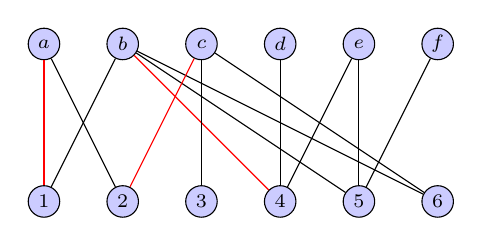
\begin{tikzpicture}[scale=1, every node/.style={circle, draw, fill=blue!20, inner sep=1pt, font=\scriptsize, minimum size=4mm}]
            \node (a) at (0, 2) {\(a\)};
            \node (b) at (1, 2) {\(b\)};
            \node (c) at (2, 2) {\(c\)};
            \node (d) at (3, 2) {\(d\)};
            \node (e) at (4, 2) {\(e\)};
            \node (f) at (5, 2) {\(f\)};

            \node (1) at (0, 0) {\(1\)};
            \node (2) at (1, 0) {\(2\)};
            \node (3) at (2, 0) {\(3\)};
            \node (4) at (3, 0) {\(4\)};
            \node (5) at (4, 0) {\(5\)};
            \node (6) at (5, 0) {\(6\)};

            \draw[red] (a) -- (1);
            \draw (a) -- (2);

            \draw (b) -- (1);
            \draw[red] (b) -- (4);
            \draw (b) -- (5);
            \draw (b) -- (6);
            
            \draw[red] (c) -- (2);
            \draw (c) -- (3);
            \draw (c) -- (6);
            
            \draw (d) -- (4);
            
            \draw (e) -- (4);
            \draw (e) -- (5);
            
            \draw (f) -- (5);
        \end{tikzpicture}
    }
}

		\begin{itemize}
			\item Je choisis \(d\) non saturé,
			\item \(6\) est non saturé donc \(d4b6\) est augmentant.
			\item On augmente \(|M|\) et on recommence.
		\end{itemize}
		
		\input{../assets/tikz/td_2_ex_9_2.tex}

		\begin{itemize}
			\item On calcule un arbre de couplage enraciné en \(3\),
			\item Il est complet, on peut le retirer du graphe
		\end{itemize}
		A la fin, il reste:

		% Figure 1
\ffigbox[\FBwidth]{%
\label{Fig:td2ex9c3}
}{
    \fbox{
        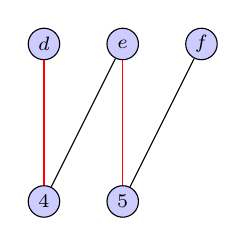
\begin{tikzpicture}[scale=1, every node/.style={circle, draw, fill=blue!20, inner sep=1pt, font=\scriptsize, minimum size=4mm}]
            \node (d) at (3, 2) {\(d\)};
            \node (e) at (4, 2) {\(e\)};
            \node (f) at (5, 2) {\(f\)};

            \node (4) at (3, 0) {\(4\)};
            \node (5) at (4, 0) {\(5\)};

            \draw[red] (d) -- (4);
            
            \draw (e) -- (4);
            \draw[red] (e) -- (5);
            
            \draw (f) -- (5);
        \end{tikzpicture}
    }
}
	\end{td-sol}
}{}


% ----- Consignes exo 10 ----- %
\begin{td-exo}[Convexité]\,\\ % 10 
	% fill
\end{td-exo}

% ----- Solutions exo 10 ----- %
\iftoggle{showsolutions}{
	\begin{td-sol}[]\,\\ %
		A remplir %TODO solve exercise 10
	\end{td-sol}
}{}


% ----- Consignes exo 11 ----- %
\begin{td-exo}[Convexité]\,\\ % 11 
	% fill
\end{td-exo}

% ----- Solutions exo 11 ----- %
\iftoggle{showsolutions}{
	\begin{td-sol}[]\,\\ %
		A remplir %TODO solve exercise 11
	\end{td-sol}
}{}


% ----- Consignes exo 12 ----- %
\begin{td-exo}[Convexité]\,\\ % 12 
	% fill
\end{td-exo}

% ----- Solutions exo 12 ----- %
\iftoggle{showsolutions}{
	\begin{td-sol}[]\,\\ %
		A remplir %TODO solve exercise 12
	\end{td-sol}
}{}


% ----- Consignes exo 13 ----- %
\begin{td-exo}[Convexité]\,\\ % 13 
	% fill
\end{td-exo}

% ----- Solutions exo 13 ----- %
\iftoggle{showsolutions}{
	\begin{td-sol}[]\,\\ %
		A remplir %TODO solve exercise 13
	\end{td-sol}
}{}


% ----- Consignes exo 14 ----- %
\begin{td-exo}[Convexité]\,\\ % 14 
	% fill
\end{td-exo}

% ----- Solutions exo 14 ----- %
\iftoggle{showsolutions}{
	\begin{td-sol}[]\,\\ %
		A remplir %TODO solve exercise 14
	\end{td-sol}
}{}

%%%%%%%%%%%%%%%%%%
% ce qu'on a vu en cours:
% - corollaire 1 de hall
% - corollaire 2 de hall